% Drawing 148/02-5 -- folder 148, batch 02, archive page 23 (PDF page 24).
% Transcription: planche de croquis, à l'encre et au crayon, sur toute la page. En haut : une sphère à trois trous ; une coupe sur un pied d'où part un petit graphe en arbre ; deux sphères à trous accolées ; un losange à quatre sommets marqués entre quatre arcs. Au milieu : une sphère à points numérotés ; deux sphères à trous ; une sphère à quatre trous ; une calotte, un petit ovale et un segment de $0$ à $1$ ; une grande sphère à l'encre épaisse (équateur portant des points, méridiens, un fuseau hachuré) reliée par une flèche à une sphère portant deux trous joints par un trait double et un troisième trou ; une petite sphère à trois trous. En bas : des ovales, des boucles au crayon, un cercle à deux trous, un grand dôme portant des points, un arc épais et des traits verts, et une sphère avec pôle, équateur et points. Trois longs traits au crayon traversent la planche de haut en bas.
% Kind: plate of sketches: spheres with holes, maps on the sphere, a rhombus, a tree. Method 2 (schematic redraw from the facsimile). Status: partial.
% Notes: Whole page, schematic: each figure is put at its place and drawn with its outline, its holes (small rings), its marked points and its heavy strokes, from the colour render at half scale; the plate gives where each sketch is and what kind it is, not its exact strokes. Kept: the rhombus with four heavy vertices between four arcs (beside « diag_Q ≃ ω_Q », which is text and not drawn); the segment 0—1; the heavy arrow between the two large spheres of the middle row; the three long pencil strokes; the two green strokes on the dome. Left out: all words and formulas (transcribed in the text), the letters a b c d written vertically, two unread curled signs (top, right of the first sphere, and middle, above the arrow), the hatching of the large middle sphere apart from a few strokes, the labels 1, 1/2 and the digits 3, 4 written on the spheres of the middle row. Still differs: positions are within two or three units; arcs inside the spheres are simplified; the small numbered sphere of the middle row left is reduced to its rings and its heavy meridian. The notes of the transcription « une sphère dont des points sont numérotés, un segment de 0 à 1 » and « un losange dont les quatre sommets sont marqués, entre deux arcs » describe parts of this plate. Redrawn 2026-11-12 (issue 128): to check again.
% Coordinates: 1 unit = 1 mm = 1/100 of the crop width, y downwards as on the crop (bbox in page fractions: [0.09, 0.07, 0.91, 0.8]).
% Redrawn by Claude (claude-fable-5-2), issue #128, 2026-11-12; not checked by a human; not compiled (no TeX in the session).
% Rights: reproduces part of the work -- behind RENDER_TRANSCRIPTS, never published by itself.
\documentclass[tikz,border=3pt]{standalone}
\usepackage{amsmath,amssymb}
\usetikzlibrary{patterns,arrows.meta}
\tikzset{pencil/.style={black!45}, struck/.style={black!35}, mpt/.style={circle,draw,inner sep=1.3pt}, pt/.style={circle,fill,inner sep=0.9pt}, opt/.style={circle,draw,fill=white,inner sep=1.1pt}, Rd/.style={red!75!black}, Gn/.style={green!45!black}, Br/.style={brown!70!black}}
\begin{document}
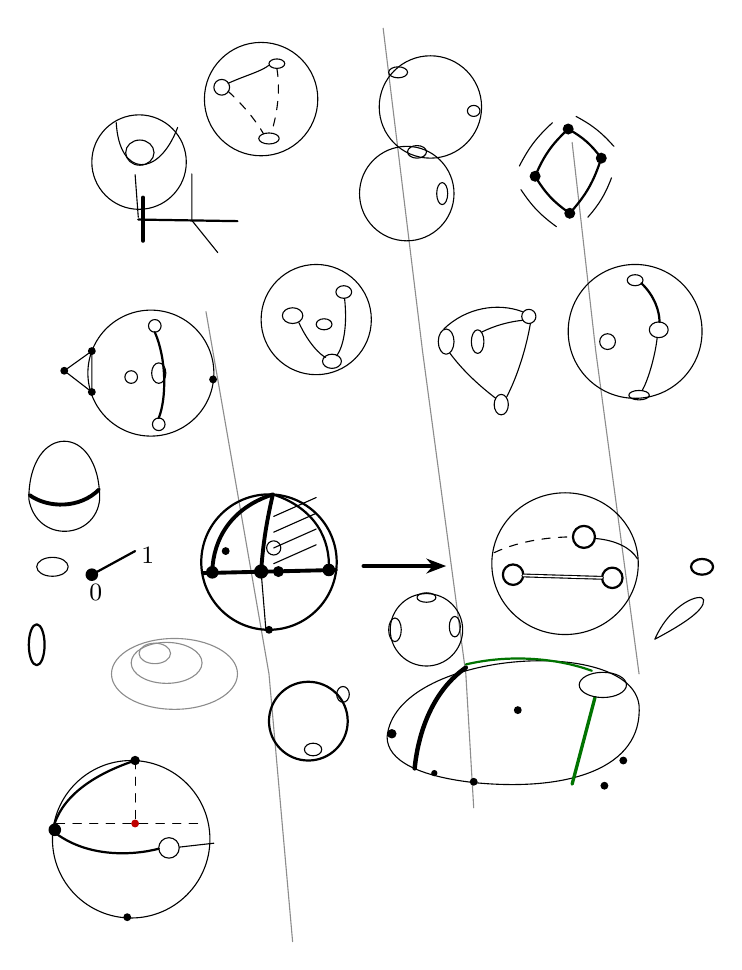
\begin{tikzpicture}[x=1mm,y=-1mm,line cap=round,line join=round,font=\small]
% three long pencil strokes
\draw[pencil] (29,45) -- (37,91) -- (40,125);
\draw[pencil] (51.5,9) -- (56.5,50) -- (62,91) -- (63,108);
\draw[pencil] (75.5,23.5) -- (78.5,50) -- (84,91);
% row 1: sphere with three holes
\draw (36,18) circle [radius=7.2];
\draw (31,16.5) circle [radius=1];
\draw (38,13.5) ellipse [x radius=1, y radius=0.6];
\draw (37,23) ellipse [x radius=1.3, y radius=0.7];
\draw[dashed] (31.8,17) .. controls (34,19) and (35.5,21) .. (36.3,22.4);
\draw[dashed] (38,14.1) .. controls (38.5,17) and (38,20) .. (37.3,22.3);
\draw (31.8,16) .. controls (34,15) and (36,14.5) .. (37,13.7);
% cup on a foot, tree
\draw (20.5,26) circle [radius=6];
\draw (17.6,21) .. controls (18,28) and (23,28) .. (25.4,21.6);
\draw (20.6,24.8) ellipse [x radius=1.8, y radius=1.6];
\draw (20,27.6) -- (20.4,33);
\draw[line width=1.4pt] (21,30.5) -- (21,36);
\draw[thick] (20.4,33.3) -- (33,33.5);
\draw (27.2,27.5) -- (27.2,33.4) -- (30.5,37.5);
% two spheres with holes
\draw (57.5,19) circle [radius=6.5];
\draw (53.4,14.6) ellipse [x radius=1.2, y radius=0.7];
\draw (63,19.5) ellipse [x radius=0.8, y radius=0.7];
\draw (55.8,24.7) ellipse [x radius=1.2, y radius=0.8];
\draw (54.5,30) circle [radius=6];
\draw (59,30) ellipse [x radius=0.7, y radius=1.4];
% rhombus between four arcs
\coordinate (r1) at (75,21.8);
\coordinate (r2) at (79.2,25.5);
\coordinate (r3) at (75.2,32.5);
\coordinate (r4) at (70.8,27.8);
\draw[thick] (r1) to[bend left=12] (r2) to[bend left=12] (r3) to[bend left=12] (r4) to[bend left=12] (r1);
\fill (r1) circle [radius=0.7];
\fill (r2) circle [radius=0.7];
\fill (r3) circle [radius=0.7];
\fill (r4) circle [radius=0.7];
\draw (68.8,26.5) to[bend left=10] (73,21);
\draw (76,20.2) to[bend left=10] (80.8,24);
\draw (80.5,28) to[bend left=10] (77.5,33);
\draw (73.5,34.2) to[bend left=10] (69,29.5);
% row 2: small sphere with numbered points
\draw (22,52.8) circle [radius=8];
\draw (22.5,46.8) circle [radius=0.8];
\draw (19.5,53.3) circle [radius=0.8];
\draw (23,52.8) ellipse [x radius=0.9, y radius=1.3];
\draw (23,59.3) circle [radius=0.8];
\draw[thick] (22.5,47.6) .. controls (24,51) and (24,56) .. (23,58.5);
\fill (29.9,53.6) circle [radius=0.5];
\draw (11,52.5) -- (14.5,50) -- (14.5,55.2) -- cycle;
\fill (11,52.5) circle [radius=0.5];
\fill (14.5,50) circle [radius=0.5];
\fill (14.5,55.2) circle [radius=0.5];
% sphere with holes (above the big one)
\draw (43,46) circle [radius=7];
\draw (40,45.5) ellipse [x radius=1.3, y radius=1];
\draw (46.5,42.5) ellipse [x radius=1, y radius=0.8];
\draw (44,46.6) ellipse [x radius=1, y radius=0.7];
\draw (45,51.3) ellipse [x radius=1.2, y radius=0.9];
\draw (40.8,46.4) .. controls (42,49) and (43.5,50.5) .. (44.2,50.8);
\draw (46.6,43.3) .. controls (47,47) and (46.4,49.5) .. (45.6,50.6);
% sphere with four holes
\draw (59.5,48.8) ellipse [x radius=1, y radius=1.6];
\draw (63.5,48.8) ellipse [x radius=0.8, y radius=1.5];
\draw (70,45.6) ellipse [x radius=0.9, y radius=0.9];
\draw (66.5,56.8) ellipse [x radius=0.9, y radius=1.3];
\draw (59.2,47.2) .. controls (62,44.5) and (66,43.8) .. (69.2,45);
\draw (60,50.3) .. controls (62,53) and (64.5,55) .. (65.8,56);
\draw (70.2,46.5) .. controls (69.6,50) and (68.4,53.5) .. (67.2,55.8);
\draw (64,47.6) .. controls (66,46.6) and (68,46.2) .. (69.2,46.1);
% sphere on the right
\draw (83.5,47.5) circle [radius=8.5];
\draw (80,48.8) circle [radius=1];
\draw (86.5,47.3) ellipse [x radius=1.2, y radius=1];
\draw (83.5,41) ellipse [x radius=1, y radius=0.7];
\draw (84,55.6) ellipse [x radius=1.3, y radius=0.6];
\draw[thick] (84.3,41.4) .. controls (86,43) and (86.6,45) .. (86.6,46.3);
\draw (86.3,48.3) .. controls (86,51) and (85,54) .. (84.4,55);
% cap, small oval, segment 0--1
\draw (6.5,68.8) .. controls (6.5,59) and (15.5,59) .. (15.5,68.8) .. controls (15,74) and (7.5,74.5) .. (6.5,68.8);
\draw[line width=1.4pt] (6.6,68.3) .. controls (9,70) and (13,70) .. (15.4,67.6);
\draw (9.5,77.4) ellipse [x radius=2, y radius=1.2];
\fill (14.5,78.4) circle [radius=0.8];
\draw[thick] (14.5,78.4) -- (20,75.4);
\node at (21.6,76) {$1$};
\node at (15,80.6) {$0$};
% large heavy sphere
\draw[thick] (37,76.8) circle [radius=8.6];
\draw[line width=1.4pt] (28.6,78.2) -- (45.5,77.8);
\draw[line width=1.4pt] (37.5,68.2) .. controls (32,70) and (30,74) .. (29.8,77.8);
\draw[line width=1.4pt] (37.5,68.2) .. controls (36.6,72) and (36.2,75) .. (36,78);
\draw[thick] (37.5,68.2) .. controls (43,70) and (44.8,74) .. (44.6,77.8);
\draw (36,78) -- (36.6,85.3);
\foreach \y in {71,73,...,77} {
\draw[thin] (37.6,\y) -- (43,\y-2.4);
}
\fill (29.8,78.1) circle [radius=0.8];
\fill (36,78) circle [radius=0.9];
\fill (38.2,78) circle [radius=0.7];
\fill (44.6,77.8) circle [radius=0.8];
\fill (31.5,75.4) circle [radius=0.5];
\fill (37,85.4) circle [radius=0.5];
\draw (37.6,75) circle [radius=0.9];
% arrow
\draw[line width=1.4pt,-{Stealth[length=2.5mm]}] (49,77.3) -- (59.5,77.3);
% sphere with two joined holes and a third
\draw (74.6,77) ellipse [x radius=9.3, y radius=9];
\draw[thick] (68,78.4) circle [radius=1.3];
\draw[thick] (80.6,78.8) circle [radius=1.3];
\draw[double] (69.3,78.5) -- (79.3,78.8);
\draw[thick] (77,73.6) circle [radius=1.4];
\draw[dashed] (65.6,75.6) .. controls (69,74) and (73,73.6) .. (75.6,73.6);
\draw (78.4,73.8) .. controls (81,74) and (83,75) .. (83.8,76.4);
% small ring, teardrop
\draw[thick] (92,77.4) ellipse [x radius=1.4, y radius=1];
\draw (86,86.6) .. controls (88,82) and (92,80.6) .. (92.2,81.6) .. controls (92.4,83) and (89,85) .. (86,86.6);
% small sphere with three holes
\draw (57,85.4) circle [radius=4.6];
\draw (53,85.4) ellipse [x radius=0.8, y radius=1.5];
\draw (60.6,85) ellipse [x radius=0.7, y radius=1.3];
\draw (57,81.3) ellipse [x radius=1.2, y radius=0.6];
% row 3: oval, pencil loops, circle with two holes
\draw[thick] (7.5,87.3) ellipse [x radius=1, y radius=2.6];
\draw[pencil] (25,91) ellipse [x radius=8, y radius=4.5];
\draw[pencil] (24,89.6) ellipse [x radius=4.5, y radius=2.6];
\draw[pencil] (22.5,88.4) ellipse [x radius=2, y radius=1.3];
\draw[thick] (42,97) circle [radius=5];
\draw (46.4,93.6) ellipse [x radius=0.8, y radius=1];
\draw (42.6,100.6) ellipse [x radius=1.1, y radius=0.8];
% dome
\draw (52,99) .. controls (53,88) and (83,86) .. (84,95) .. controls (84.5,103) and (75,106) .. (63,104.8) .. controls (56,104) and (52,102) .. (52,99);
\draw[line width=1.6pt] (62,90.2) .. controls (58,93) and (56,98) .. (55.5,103);
\draw[Gn,thick] (62,89.8) .. controls (67,88.6) and (73,88.8) .. (78,90.6);
\draw[Gn,very thick] (78.4,94) -- (75.5,105);
\draw (79.4,92.4) ellipse [x radius=3, y radius=1.6];
\fill (52.6,98.6) circle [radius=0.6];
\fill (68.6,95.6) circle [radius=0.5];
\fill (63,104.7) circle [radius=0.5];
\fill (82,102) circle [radius=0.5];
\fill (79.6,105.2) circle [radius=0.5];
\fill (58,103.6) circle [radius=0.4];
% sphere with pole and equator
\draw (19.5,112) circle [radius=10];
\fill (20,102) circle [radius=0.6];
\draw[thick] (20,102) .. controls (14,104) and (10.5,107) .. (9.6,110.6);
\draw[thick] (9.6,111) .. controls (14,114.5) and (20,114) .. (23,113.2);
\draw (25.6,113) -- (30,112.5);
\draw (24.3,113.1) circle [radius=1.3];
\draw[dashed] (10,110) -- (28,110);
\draw[dashed] (20,102) -- (20,110);
\fill[Rd] (20,110) circle [radius=0.5];
\fill (9.8,110.8) circle [radius=0.8];
\fill (19,121.9) circle [radius=0.5];
\end{tikzpicture}
\end{document}
